\documentclass[a4paper,12pt]{extarticle}
\usepackage{geometry}
\usepackage[T1]{fontenc}
\usepackage[utf8]{inputenc}
\usepackage[english,russian]{babel}
\usepackage{amsmath}
\usepackage{amsthm}
\usepackage{amssymb}
\usepackage{fancyhdr}
\usepackage{setspace}
\usepackage{graphicx}
\usepackage{colortbl}
\usepackage{tikz}
\usepackage{pgf}
\usepackage{subcaption}
\usepackage{listings}
\usepackage{indentfirst}
\usepackage[
backend=biber,
style=numeric,
maxbibnames=99
]{biblatex}
\addbibresource{refs.bib}
\usepackage[colorlinks,citecolor=blue,linkcolor=blue,bookmarks=false,hypertexnames=true, urlcolor=blue]{hyperref} 
\usepackage{indentfirst}
\usepackage{mathtools}
\usepackage{booktabs}
\usepackage[flushleft]{threeparttable}
\usepackage{tablefootnote}

\usepackage{chngcntr} % нумерация графиков и таблиц по секциям
\counterwithin{table}{section}
\counterwithin{figure}{section}

\graphicspath{{graphics/}}%путь к рисункам

\makeatletter
% \renewcommand{\@biblabel}[1]{#1.} % Заменяем библиографию с квадратных скобок на точку:
\makeatother

\geometry{left=2.5cm}% левое поле
\geometry{right=1.0cm}% правое поле
\geometry{top=2.0cm}% верхнее поле
\geometry{bottom=2.0cm}% нижнее поле
\setlength{\parindent}{1.25cm}
\renewcommand{\baselinestretch}{1.5} % междустрочный интервал


\newcommand{\bibref}[3]{\hyperlink{#1}{#2 (#3)}} % biblabel, authors, year
\addto\captionsrussian{\def\refname{Список литературы (или источников)}} 

\renewcommand{\theenumi}{\arabic{enumi}}% Меняем везде перечисления на цифра.цифра
\renewcommand{\labelenumi}{\arabic{enumi}}% Меняем везде перечисления на цифра.цифра
\renewcommand{\theenumii}{.\arabic{enumii}}% Меняем везде перечисления на цифра.цифра
\renewcommand{\labelenumii}{\arabic{enumi}.\arabic{enumii}.}% Меняем везде перечисления на цифра.цифра
\renewcommand{\theenumiii}{.\arabic{enumiii}}% Меняем везде перечисления на цифра.цифра
\renewcommand{\labelenumiii}{\arabic{enumi}.\arabic{enumii}.\arabic{enumiii}.}% Меняем везде перечисления на цифра.цифра


% new math commands
\let\b\relax
\newcommand{\b}{\mathbf}
\newcommand{\R}{\mathbb{R}}

\begin{document}
\begin{titlepage}
\newpage

{\setstretch{1.0}
\begin{center}
ПРАВИТЕЛЬСТВО РОССИЙСКОЙ ФЕДЕРАЦИИ\\
ФГАОУ ВО НАЦИОНАЛЬНЫЙ ИССЛЕДОВАТЕЛЬСКИЙ УНИВЕРСИТЕТ\\
«ВЫСШАЯ ШКОЛА ЭКОНОМИКИ»
\\
\bigskip
Факультет компьютерных наук\\
Образовательная программа «Прикладная математика и информатика»
\end{center}
}


\begin{center}
%Выберите какой у вас проект
{\bf Отчет о командном исследовательском проекте на тему:}\\
%{\bf Отчет о командном программном проекте на тему:}\\
{\bf Разработка программы гарантированного нахождения глобального минимума функции}
(промежуточный, этап 1)
\end{center}

\vspace{2em}

{\bf Выполнили студенты: \vspace{2mm}}

{\setstretch{1.1}
\begin{tabular}{l@{\hskip 1.5cm}l}
группы \#БПМИ229 & Леонтьев Константин Валерьевич \\
группы \#БПМИ229 & Резниченко Александр Владиславович \\
группы \#БПМИ229 & Рудавский Владимир Владимирович
\end{tabular}}

\vspace{1em}
{\bf Принял руководитель проекта: \vspace{2mm}}

{\setstretch{1.1}
\begin{tabular}{l@{\hskip 1.5cm}l}
Посыпкин Михаил Анатольевич \\
Штатный преподаватель (ИЛИ ПРОФЕССОР? Или заведующий?)\\
Базовая кафедра
"Интеллектуальные технологии системного анализа и управления"\\
ФИЦ "Информатика и управление" РАН
\end{tabular}}

\vspace{\fill}

\begin{center}
Москва 2024
\end{center}

\end{titlepage}% это титульный лист - выберите подходящий вам из имеющихся в проекте вариантов
\newpage
\setcounter{page}{2}

{
	\hypersetup{linkcolor=black}
	\tableofcontents
}

\newpage

\newpage
\section*{Аннотация}   % this is how to use russian
В данной работе описывается создание библиотеки на языке Python для решения задачи глобальной оптимизации с использованием интервальных методов.

\addcontentsline{toc}{section}{Аннотация}

\section*{Ключевые слова}
Интервальный анализ, глобальная оптимизация, интервальное расширение, гарантированный поиск, Python
\pagebreak

\section{Введение} 
Целью данной работы является создание библиотеки для решения задачи глобальной оптимизации, которую можно сформулировать следующим образом: для вещественнозначной функции $f : \b{X} \to \R$ на брусе $\b{X} \subset \R^{n}$ с гранями, параллельными координатным осям, найти $\inf_{x \in \b{X}} f(x)$~\cite{interval-analysis-intro}.

Данная задача появляется во многих областях, например, в экономике, статистике, обработке изображений, химии, биологии~\cite{horst2000introduction}. При этом интервальный подход к её решению имеет значительное преимущество над другими: для его применения не обязательно знать свойства функции, такие как, например, выпуклость. К тому же он может быть использован для вычисления на компьютере.

Несмотря на это, на языке Python в открытом доступе нет библиотек, реализующих интервальные методы глобальной оптимизации, в этом заключается актуальность данной работы.

В задачи проекта входит:
\begin{enumerate}
	\item Изучение методов глобальной оптимизации на основе интервального анализа,
	\item Реализация различные способы оценки функции на заданном параллелепипеде,
	\item Разработка тесты для проверки эффективности созданных решений,
	\item Проведение тестирования и формирование выводов об эффективности предложенных решений.
\end{enumerate}


\pagebreak
% \section{Примеры} 
% \subsection{Ссылки на статьи}

% Ссылки на статьи оформляются с помощью пакета \texttt{biblatex}, например~\cite{chirkova18}. В описании статье в bib файле нужно обязательно указывать место публикации работы (журнал или конференцию) и год. Обратите внимание, что для описания статей из разных источников в списке литературы используются разные команды в bib файле: статья из журнала~\cite{ctan}, статья с конференции~\cite{chirkova18}, книга~\cite{knuth-acp}, глава книги~\cite{knuth-fa}. Если статься еще не опубликована нигде, а только выложена на arXiv, то на нее тоже можно сослаться~\cite{chirkova18_arxiv}, но предпочтительно ссылаться на опубликованную версию, если она уже существует. Если вы хотите сослаться на сайт, то можно либо так же внести его в список литературы~\cite{knuthwebsite} (рекомендуется, если таких ссылок у вас много из-за особенностей темы вашего проекта), либо использовать ссылку внизу страницы\footnote{Книги доступны по ссылке: \url{http://www-cs-faculty.stanford.edu/~uno/abcde.html}, дата обр. 16.05.2013}. При работе с онлайн ресурсами не забывайте указывать дату обращения к этому ресурсу, так как в отличие от опубликованных статей, эти ресурсы могут измениться в любой момент.

% \subsection{Рисунки}

% \begin{figure}[ht]
% 	\centering
% 	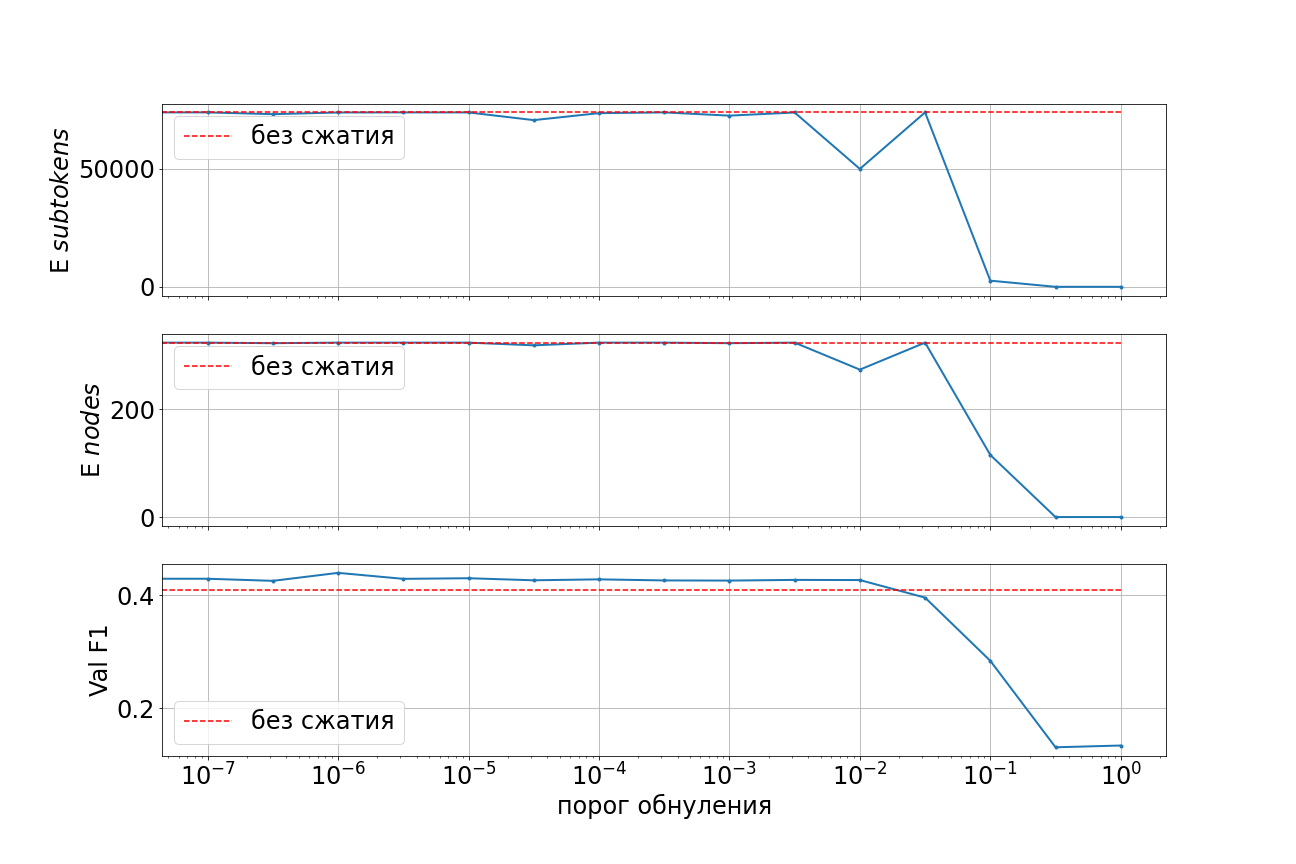
\includegraphics[width=0.8\textwidth]{example.png}
% 	\caption{Пример графика. Тут должна быть подпись, поясняющая что происходит на рисунке (краткая, но достаточная для понимания основной идеи графика).}
% 	\label{fig:by_epochs}
% \end{figure}

% Все рисунки в тексте должны иметь подписи и вы на них должны ссылаться в тексте. Например, на Рисунке~\ref{fig:by_epochs} изображен пример графика. Не забывайте подписывать все оси на графиках, добавлять легенду и пояснять все обозначения, а также используйте адекватного размера шрифты и толщину линий на графиках (все должно быть видно и понятно без многократного увеличения). На рисунке из примера явно не хватает обозначения синей линии в легенде.


% \subsection{Таблицы}

% Все таблицы в тексте тоже должны иметь подписи и вы на них должны ссылаться в тексте. Например, в Таблице~\ref{table:long_epochs} показаны результаты примерного эксперимента. 


% \begin{table}[ht]
% 	\caption{Пример таблички. Тут должна быть подпись, поясняющая что происходит в таблице (краткая, но по делу).}
% 	\label{table:long_epochs}
% 	\footnotesize
% 	\centering
% 	\begin{tabular}{lrrrrrrrr}
% 		\toprule
% 		& \multicolumn{3}{c}{$\mathsf{Val}$} &
% 		\multicolumn{3}{c}{$\mathsf{Test}$} \\
% 		\cmidrule(lr){2-4} \cmidrule(l){5-7} 
% 		{} &  $\mathsf{Prec}$ &  $\mathsf{Rec}$ &  $\mathsf{F1}$ &  $\mathsf{Prec}$ &  $\mathsf{Rec}$ &  $\mathsf{F1}$  &  $\mathsf{nodes}$ & $\mathsf{subtokens}$\\
% 		\midrule
% 		запуск 1    &    0.4894 &   0.3775 &  0.4263 &     0.4824 &    0.3683 &   0.4177 & 10029 & 179\\
% 		запуск 2    &    0.4887 &   0.3739 &  0.4237 &     0.4891 &    0.3724 &   0.4228 & 10039 & 177\\
% 		запуск 3    &    0.4820 &   0.3751 &  0.4219 &     0.4838 &    0.3677 &   0.4178 & 10037&	180\\
% 		\midrule
% 		\bf{среднее} &    \bf{0.4867} &   \bf{0.3755} &  \bf{0.4239} &    \bf{ 0.4851} &    \bf{0.3695} &   \bf{0.4195} \\
% 		\bf{дисперсия}  &    0.0041 &   0.0019 &  0.0022 &     0.0036 &    0.0025 &   0.0029 \\
% 		\bottomrule
% 	\end{tabular}
% \end{table}

% \subsection{Формулы}

% Формулы стоит центрировать, а также нумеровать, если вы ссылаете на них в тексте. Также не забывайте пояснять все обозначения в формулах. Например, запишем следующую задачу оптимизации:
% \begin{equation}
%     \label{eq:si_opt}
%         \theta* = \min_{\theta} F(\theta),
% \end{equation}
% где $F$~-- квадратичная функция от параметра $\theta$. При необходимости, далее в тексте можно сослаться на формулу~(\ref{eq:si_opt}). При этом, в зависимости от конкретных формул, можно использовать разные слова: формула, уравнение, задача оптимизации и т.п.


\section*{Реализация}
\subsection*{Обработка данных и внутреннее представление}
Для парсинга математических функций была использована библиотека sympy~\cite{python-sympy}. В частности функция parse\_expr, преобразующая строку в дерево выражений, каждое из которых является объектом одного из классов sympy. Поскольку sympy не поддерживает вычисления от произвольных типов, полученная структура приводится к внутреннему представлению: дереву, в вершинах которого содержатся функция и аргументы.

Далее дерево может быть использовано для получения естественного расширения функции, так как поддерживает вычисления от любого типа, для которого реализованы арифметические операции и элементарные функции. К тому же, в дальнейшем структура может быть использована для автоматического дифференцирования.

Для работы с числами был использован модуль decimal~\cite{python-decimal}, позволяющий задавать не только произвольную точность, но и тип округления вычислений, что необходимо для построения внешней интервальной оценки.

Для получения интервального расширения логарифма и экспоненты были использованы методы, предоставленные модулем decimal. Поскольку они позволяют найти ответ только с округлением в ближайшему чётному, наш алгоритм итеративно повышает точность вычисления, пока интервал, в котором лежит ответ, не определён однозначно. В модуле отсутствуют тригонометрические функции, потому их реализация потребует написания приближения рядом Тейлора.

Интерфейс библиотеки состоит из одного метода get\_extremum\_estimation. Он позволяет найти минимум или максимум функции на заданном брусе. При этом пользователь может задать необходимую точность ответа, тип интервального расширения и метод глобальной оптимизации.

Эту часть системы реализовал Владимир Рудавский.

\section{План выполнения работы}
\subsection*{Основной план}
\begin{enumerate}
	\item Реализовать естественное интервальное расширение функций (сделал Владимир Рудавский) 
	\item Реализовать алгоритм Мура-Скелбоя (сделал Александр Резниченко)
	\item Разработать тестирующую систему для функций поиска глобального экстремума (сделал Константин Леонтьев)
	\item Реализовать оптимизации алгоритма Мура-Скелбоя, в том числе удаление брусков, заведомо не содержащих точку экстреумуа, подсчёт частных производных для определения оптимальной координаты дробления (ПРИДУМАЙ ЕЩЕ КАКИЕ-НИБУДЬ) (сделает Александр Резниченко)
	\item Реализовать алгоритм отжига для поиска глобального минимума (сделает Александр Резниченко)
	\item Реализовать автоматическое дифференцирование (сделает Владимир Рудавский)
	\item Реализовать построение центрированных и бицентрированных форм (сделает Владимир Рудавский)
	\item Расширить количество тестов для функций поиска глобального экстремума (сделает Леонтьев Константин)
	\item ТАК ТУТ НАДО ЕЩЕ АЛГОСЫ КАКИЕ-НИБУДЬ НАЙТИ и приписать Косте
\end{enumerate}

	
\newpage 
\printbibliography[heading=bibintoc] 

% \begin{thebibliography}{0}
% 	\bibitem{chirkova18}\hypertarget{chirkova18}{}
% 	\href{https://arxiv.org/abs/1810.10927}
% 	{Nadezhda Chirkova, Ekaterina Lobacheva, Dmitry Vetrov. Bayesian Compression for Natural Language Processing. In EMNLP 2018.}
% \end{thebibliography}
	
	
\end{document}
